\documentclass[9pt,handout]{beamer}

\input{StyleFile.tex}

% \setbeameroption{show notes}
% \setbeameroption{show notes on second screen=right}

\title[\textbf{Resilient Machine Learning Approaches for Fast Risk Evaluation and Management in Financial Portfolios and Variable Annuities}]{Efficient Machine Learning Approaches for Fast Risk Evaluation of VAs}

\author[\textbf{Xintong Li, xintong.li1@uwaterloo.ca}]
{\Large\bfseries
Xintong Li\\\medskip
xintong.li1@uwaterloo.ca
} % Your name

\institute[\textbf{University of Waterloo, Actuarial Science}] % Your institution as it will appear on the bottom of every slide, may be shorthand to save space
{\large\bfseries
Dept. Statistics and Actuarial Science\\\smallskip
University of Waterloo % Your institution for the title page
}


\jointwork{Supervised by Prof. Tony Wirjanto and Prof. Mingbin Feng}
\conference{Thesis Defense, University of Waterloo}


%\usepackage[backend=bibtex,citestyle=authoryear-icomp,natbib,maxcitenames=1]{biblatex}
%\addbibresource{NestedSim.bib}

% use this so appendices' page numbers do not count
\usepackage{appendixnumberbeamer}
\usepackage{booktabs}
\usepackage{subfigure}
\usepackage[round]{natbib}
\usepackage{mathtools}


\usepackage{amsmath}
\usepackage{amsfonts}
\usepackage{amssymb}
\usepackage{bbm}
\usepackage{xcolor}
\usepackage{algorithm}
\usepackage{algpseudocode}
\usepackage{algorithmicx}
\usepackage{multirow}
\usepackage{graphicx}

\usepackage{tikz}
\usetikzlibrary{decorations.pathreplacing}


\newcommand{\E}{\mathbb{E}}
\newcommand{\R}{\mathbb{R}}
\newcommand{\I}{\mathbbm{1}}

\newcommand{\fracM}{\frac{1}{M}}
\newcommand{\fracMM}{\frac{1}{M^2}}
\newcommand{\sumM}{\sum_{i=1}^M}

\newcommand{\fracN}{\frac{1}{N}}
\newcommand{\fracNN}{\frac{1}{N^2}}
\newcommand{\sumN}{\sum_{j=1}^N}

\newcommand{\rhoh}{\hat{\rho}}
\newcommand{\Lh}{\hat{L}}
\newcommand{\betah}{\hat{\beta}}

\newcommand{\Bias}{\textnormal{Bias}}
\newcommand{\Variance}{\textnormal{Variance}}

\newcommand{\SNS}{\textnormal{SNS}}
\newcommand{\REG}{\textnormal{REG}}
\newcommand{\KS}{\textnormal{KS}}
\newcommand{\LR}{\textnormal{LR}}
\newcommand{\KRR}{\textnormal{KRR}}
\newcommand{\skipv}{\vspace{8pt}}


\newtheorem{assumption}{Assumption}
\newtheorem{proposition}{Proposition}

\DeclarePairedDelimiter\ceil{\lceil}{\rceil}
\DeclarePairedDelimiter\floor{\lfloor}{\rfloor}

\begin{document}

% Title page, navigation surpressed, no page number
{
\beamertemplatenavigationsymbolsempty
\begin{frame}[plain]
\titlepage
\end{frame}
}

{
\beamertemplatenavigationsymbolsempty
\defbeamertemplate*{headline}{miniframes theme no subsection no content}
{ \begin{beamercolorbox}{section in head/foot}
    \vskip\headheight
  \end{beamercolorbox}}
\begin{frame}{Outline}
\tableofcontents
\end{frame}
}
\addtocounter{framenumber}{-2}

\section{Introduction}

\begin{frame}{Nested Simulation Procedures}

Nested simulation procedures are necessary for \textbf{complex} financial derivatives and insurance products.

$$\rho(L) = \rho(L(X)), \;\;\; L(X) = \mathbb{E}\left[ Y|X=x \right]\vert_{x=X}  $$

Involves two levels of Monte Carlo simulations:
\begin{itemize}
    \item Outer level: generates underlying risk factors (outer scenarios), $X_i \sim F_X$
    \item Inner level: generates scenario-wise samples of portfolio losses (inner replications), $Y_{ij} \sim F_{Y|X_i}$
\end{itemize}

\textbf{Computationally expensive due to its nested structure.}

\end{frame}

\begin{frame}{Common Risk Measures}

\begin{itemize}
    \item Smooth $h$, e.g., quadratic tracking error

    $$ \rho(L) = \mathbb{E} \left[ (L - b)^2 \right] $$
    
    \item hockey-stick $h$: mean excess loss
    
    $$ \rho(L) = \mathbb{E} \left[ L \cdot \mathbbm{1}_{\{L \geq u\}} \right] $$
    
    \item indicator $h$: probability of large loss
    
    $$ \rho(L) = \mathbb{E} \left[ \mathbbm{1}_{\{L \geq u\}} \right] $$
    
    \item Value at Risk (VaR)
    
    $$ \rho_\alpha(L) = Q_\alpha(L) = \inf \{ u: \mathbb{P}(L \leq u) \geq \alpha \} $$
    
    \item Conditional Value at Risk (CVaR) \footnotemark
    
    $$ \rho_\alpha(L) = \mathbb{E} \left[ L \vert L \geq Q_\alpha(L) \right] $$

    \end{itemize}

    \footnotetext{Note: If $Q_\alpha(L)$ falls in a probability mass, $\rho(L) = \frac{(\beta - \alpha)Q_\alpha(L) + (1- \beta) \mathbb{E} \left[ L \vert L \geq Q_\alpha(L) \right]}{1-\alpha}$.}

\end{frame}

\section{Nested Simulation Procedures in Financial Engineering: A Selected Review}

\begin{frame}{Standard Nested Simulation}

$$\hat{L}_{N, i} = \frac{1}{N} \sum_{j=1}^N Y_{ij}; ~~~ Y_{ij} \sim F_{Y|X_i} $$

\begin{itemize}
    \item Uses inner sample mean to estimate $L(X_i)$.
    \item Proposed by \citet{gordy2010nested}; finds optimal growth order of $M$ and $N$.
    \item \citet{zhang2021bootstrap} estimate the optimal $M$ and $N$ using a bootstrap method.
    \item Computationally expensive and potentially \textbf{wasteful} use of budget.
\end{itemize}

\end{frame}

\begin{frame}{Other Nested Simulation Procedures}

Subsequent works focus on improving the efficiency of nested simulation:
\begin{itemize}
    \item Regression-based~\citep{broadie2015risk}
    \item Kernel smoothing~\citep{hong2017kernel}
    \item Likelihood ratio~\citep{feng2020optimal}
    \item Kernel ridge regression~\citep{zhang2022sample}
\end{itemize}

\vspace{10pt}

\textbf{Key ideas:} 
\begin{itemize}
    \item Pool inner replications from different outer scenarios 
    \item Use metamodeling techniques to approximate the inner simulation model
\end{itemize}

\end{frame}

\begin{frame}{Metamodeling Approach}

In this thesis, we focus on procedures that use \textbf{supervised learning metamodels} to approximate the inner simulation model.   

\begin{itemize}
    \item Treat the inner simulation as a black-box function
    \item Approximate $L(\cdot)$ with $\hat{L}^{\text{SL}}_{M, N}(\cdot)$
    \item Train with a set of feature-label pairs generated from the standard procedure:
    $$\{(X_i, \hat{L}_{N, i}) \vert i=1, \ldots, M, j=1, \ldots, N\}$$
    \item Use trained metamodel to make predictions for all $X \in \mathcal{X}$
\end{itemize}

There are \textbf{computational costs} associated with pooling inner replications.

\end{frame}

\begin{frame}{Problem Statement}

Minimize mean squared error (MSE) of the estimator subject to total simulation budget:

\begin{align*}
\min_{M, N} ~~~ \mathbb{E} \left[ \left( \hat{\rho}_{M, N} - \rho \right)^2 \right] \\
\text{ subject to } M \cdot N = \Gamma
\end{align*}

Interested in convergence order as $\Gamma \to \infty$

\end{frame}

\subsection{Theoretical Results}

\begin{frame}{Asymptotic Convergence Rates of Different Procedures}

    \begin{table}
		\centering
		\begin{tabular}{l|c|c|c}
			\toprule
			\textbf{Procedures} & \textbf{Smooth $h$} & \textbf{Hockey-Stick $h$} & \textbf{Indicator $h$}  \\
			\midrule
			Standard Procedure	& \textcolor{red}{$\mathcal{O}(\Gamma^{-2/3})$} & \textcolor{red}{$\mathcal{O}(\Gamma^{-2/3})$} & $\mathcal{O}(\Gamma^{-2/3})$ \\
			\midrule
			Regression  & $\mathcal{O}(\Gamma^{-1})$ & $\mathcal{O}(\Gamma^{-1+\delta})$ & No Result \\
			\midrule
			Kernel Smoothing 	& \multicolumn{3}{c}{$\mathcal{O}(\Gamma^{-\min(1, 4/(d+2))})$}  \\
			\midrule
			Kernel Ridge Regression  		& \multicolumn{3}{c}{$\mathcal{O}(\Gamma^{-1})$} \\
			\midrule
			Likelihood Ratio  			& \multicolumn{3}{c}{$\mathcal{O}(\Gamma^{-1})$} \\
			\bottomrule
		\end{tabular}
	\end{table}
    \vspace{10pt}
    \begin{itemize}
        \item We show the asymptotic convergence rates of the standard procedure for smooth and hockey-stick $h$.
        \item Only kernel smoothing depends on the asset dimension $d$.
    \end{itemize}
    
\end{frame}

\begin{frame}{Key Theoretical Results}

\textbf{Observations:}
\begin{itemize}
\item Most literature focuses on the MSE of $\hat{\rho}$.
\item \citet{wang2022smooth} analyze convergence of absolute error in probabilistic order.
\end{itemize}

\vspace{10pt}

\textbf{Contribution:} bridging the gap between MSE and absolute error convergence.
\begin{itemize}
    \item Convergence in MSE:
    $$ \mathbb{E} \left[ \left( \hat{\rho}_{\Gamma} - \rho \right)^2 \right] = \mathcal{O} \left( \Gamma^{-\xi} \right) $$
    \item Convergence in Probabilistic Order:
    $$ |\hat{\rho}_{\Gamma} - \rho| = \mathcal{O}_{\mathbb{P}}(\Gamma^{-\xi}) $$
\end{itemize}

\end{frame}

\begin{frame}{Key Theoretical Results}

\begin{block}{Theorem}
    If $\hat{\rho}_{\Gamma}$ converges in MSE to $\rho$ in order $\xi$, then $\hat{\rho}_{\Gamma}$ converges in probabilistic order to $\rho$ in order $\frac{\xi}{2}$.
\end{block}

\begin{itemize}
    \item First result to draw connection between MSE and probabilistic order convergence.
    \item Applicable to any nested simulation procedure.
    \item Convergence in MSE implies convergence in probabilistic order.
\end{itemize}

\end{frame}

\subsection{Finite-Sample Analysis}

\begin{frame}{Experiment Design}

We compare 5 nested simulation procedures 
\begin{itemize}
    \item Standard nested simulation
    \item Regression-based
    \item Kernel smoothing
    \item Likelihood ratio
    \item Kernel ridge regression
\end{itemize}

And their empirical convergence stable across different:
\begin{itemize}
    \item Risk measures
    \item Option types
    \item Asset dimensions
    \item Asset models (GBM vs. Heston)
    \item Regression bases (only for the regression-based procedure)
\end{itemize}

\end{frame}

\begin{frame}{Finite-Sample Performance}

\begin{figure}
    \includegraphics[width=\textwidth]{../project1/figures/figure1.png}
    \caption{Empirical convergence rates of different procedures for the base case}
\end{figure}

\end{frame}

\begin{frame}{Sensitivity to Asset Dimension}

\begin{figure}
    \includegraphics[width=\textwidth]{../project1/figures/figure2a.png}
\end{figure}

\begin{itemize}
    \item Standard, KRR, and likelihood ratio procedures are dimension-independent
    \item Kernel smoothing and regression show sensitivity to dimension, but in different ways
\end{itemize}

\end{frame}

\begin{frame}{Sensitivity to Asset Dimension}

    \begin{figure}
        \includegraphics[width=\textwidth]{../project1/figures/figure2b.png}
    \end{figure}
    
    \begin{itemize}
        \item Standard, KRR, and likelihood ratio procedures are dimension-independent
        \item Kernel smoothing and regression show sensitivity to dimension, but in different ways
    \end{itemize}
    
\end{frame}

\begin{frame}{Fast Convergence of Regression-based Procedure}

\begin{figure}
    \includegraphics[width=\textwidth]{../project1/figures/figure3.png}
\end{figure}

\begin{itemize}
    \item Higher initial convergence rate
    \item Stabilizes to match asymptotic rate at higher budgets
    \item Consistent across different asset dimensions
\end{itemize}

\end{frame}

\begin{frame}{Sensitivity to Option Type}

\begin{figure}
    \includegraphics[width=\textwidth]{../project1/figures/figure6a.png}
\end{figure}

\begin{itemize}
    \item Similar convergence patterns across different option types
    \item Regression and kernel smoothing show higher empirical rates for barrier options
\end{itemize}

\end{frame}

\begin{frame}{Sensitivity to Risk Measure}

\begin{figure}
    \includegraphics[width=\textwidth]{../project1/figures/figure8a.png}
\end{figure}

\begin{itemize}
    \item Convergence behavior consistent across different risk measures
    \item Regression-based method shows highest empirical convergence rates
\end{itemize}

\end{frame}

\begin{frame}{Sensitivity to VaR/CVaR Level}

\begin{figure}
    \includegraphics[width=\textwidth]{../project1/figures/figure9a.png}
\end{figure}

\begin{itemize}
    \item Regression-based method not sensitive to VaR/CVaR level
    \item Consistent performance across different levels
\end{itemize}

\end{frame}

\begin{frame}{Sensitivity to Asset Model}

\begin{figure}
    \includegraphics[width=\textwidth]{../project1/figures/figure10a.png}
\end{figure}

\begin{itemize}
    \item Regression-based method insensitive to asset model (GBM vs. Heston)
    \item Consistent performance across different asset models
\end{itemize}

\end{frame}

\begin{frame}{Computational Complexity}

    There are \textbf{computational costs} associated with pooling inner replications.

    \begin{itemize}
        \item Standard procedure: cost of estimating the optimal $M$ and $N$
        \item Regression: most efficient among metamodel-based procedures
        \item Kernel smoothing: costly distance calculations and cross-validation
        \item Likelihood ratio: No training, but costly weight calculations
        \item KRR: even more expensive than kernel smoothing
    \end{itemize}

\end{frame}

\begin{frame}{Total Computation Time}

    \begin{figure}
        \includegraphics[width=\textwidth]{../project1/figures/figure11b.png}
        \caption{Total computation time for different procedures}
    \end{figure}

\end{frame}

\begin{frame}{Cost of Hyperparameter Tuning}

    \begin{figure}
        \includegraphics[width=\textwidth]{../project1/figures/figure12a.png}
        \caption{Cost of hyperparameter tuning for different procedures}
    \end{figure}

\end{frame}

\begin{frame}{Cost of Model Fitting and Validation}

    \begin{figure}
        \includegraphics[width=\textwidth]{../project1/figures/figure12b.png}
        \caption{Cost of model fitting and validation for different procedures}
    \end{figure}

\end{frame}

\begin{frame}{Conclusion}
    Regression-based nested simulation procedure:
    \begin{itemize}
        \item Most robust and stable for limited budgets
        \item Efficient to implement
        \item Fast empirical convergence for option portfolios
    \end{itemize}

    \vspace{10pt}

    For high-dimensional or complex payoffs:
    \begin{itemize}
        \item Difficult to find a good regression basis
        \item Neural network-based procedures may be more suitable
    \end{itemize}

    \vspace{10pt}

    Next project: examining performance of metamodel-based simulation procedures for variable annuities


\end{frame}

\section{Using Deep Neural Network Metamodels for High-Dimensional Nested Simulation}

\begin{frame}{From Options to Variable Annuities}

    Variable annuities (VAs) poses a challenge for nested simulation due to its \textbf{high-dimensional} and \textbf{complex payoff structure}.

    \begin{figure}[H]
        \makebox[\textwidth][c]{
            \subfigure{
                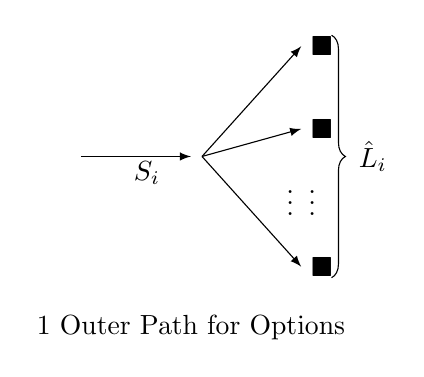
\begin{tikzpicture}[scale=0.7]
                \draw[-latex] (0,0)--(2,0);
                \draw[-latex] (2.2,0)--(4,2) node[right]  {$\blacksquare$};
                \draw[-latex] (2.2,0)--(4,0.5) node[right]  {$\blacksquare$};
                \draw[-latex] (2.2,0)--(4,-2) node[right]  {$\blacksquare$};
                \node at (1.2,-0.3) {$S_i$};
                \node at (3.8,-0.7) {$\vdots$};
                \node at (4.2,-0.7) {$\vdots$};
                \draw [decorate,  decoration = {brace,    raise=1pt,    amplitude=5pt}] (4.5,2.2) --  (4.5,-2.2);
                \node at (5.3,0) {$\hat L_i$};
                \node at (2,-3.1) {1 Outer Path for Options};
                \end{tikzpicture}}
            \subfigure{
                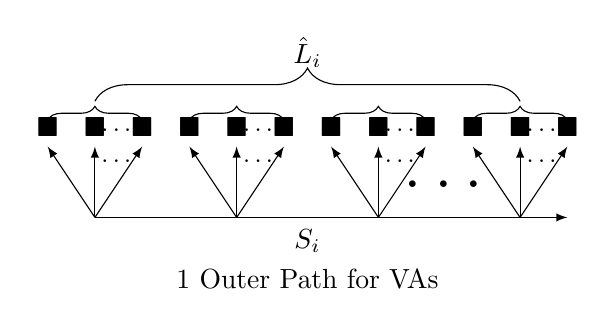
\begin{tikzpicture}[scale=0.6]
                \draw[-latex] (0,0)--(10,0);
                \draw[-latex] (0,0)--(-1,1.5) node[above] {$\blacksquare$};
                \draw[-latex] (0,0)--(0,1.5) node[above] {$\blacksquare$};
                \draw[-latex] (0,0)--(1,1.5) node[above] {$\blacksquare$};
                \node at (0.5,1.2) {\small$\dots$};
                \node at (0.5,1.85) {\small$\dots$};
                
                \draw[-latex] (3,0)--(2,1.5) node[above] {$\blacksquare$};
                \draw[-latex] (3,0)--(3,1.5) node[above] {$\blacksquare$};
                \draw[-latex] (3,0)--(4,1.5) node[above] {$\blacksquare$};
                \node at (3.5,1.2) {\small$\dots$};
                \node at (3.5,1.85) {\small$\dots$};
                
                \draw[-latex] (6,0)--(5,1.5) node[above] {$\blacksquare$};
                \draw[-latex] (6,0)--(6,1.5) node[above] {$\blacksquare$};
                \draw[-latex] (6,0)--(7,1.5) node[above] {$\blacksquare$};
                \node at (6.5,1.2) {\small$\dots$};
                \node at (6.5,1.85) {\small$\dots$};
                
                \draw[-latex] (9,0)--(8,1.5) node[above] {$\blacksquare$};
                \draw[-latex] (9,0)--(9,1.5) node[above] {$\blacksquare$};
                \draw[-latex] (9,0)--(10,1.5) node[above] {$\blacksquare$};
                \node at (9.5,1.2) {\small$\dots$};
                \node at (9.5,1.85) {\small$\dots$};
                
                \node at (7.5,0.7) {\Huge $\dots$};
                
                \draw [decorate,  decoration = {brace,    raise=1pt,    amplitude=5pt}] (-1,2) --  (1,2);
                \draw [decorate,  decoration = {brace,    raise=1pt,    amplitude=5pt}] (2,2) --  (4,2);
                \draw [decorate,  decoration = {brace,    raise=1pt,    amplitude=5pt}] (5,2) --  (7,2);
                \draw [decorate,  decoration = {brace,    raise=1pt,    amplitude=5pt}] (8,2) --  (10,2);
                \draw [decorate,  decoration = {brace,    raise=1pt,    amplitude=12pt}] (0,2.4) --  (9,2.4);
                \node at (4.5,-0.5) {$S_i$};
                \node at (4.5,3.5) {$\hat L_i$};
                \node at (4.5,-1.3) {1 Outer Path for VAs};
                \end{tikzpicture}
                }}
	\end{figure}

    \begin{itemize}
        \item Need to reconstruct a metamodeling-based nested simulation procedure
    \end{itemize}

\end{frame}

\begin{frame}{Nested Simulation for Risk Management of VAs}

    \begin{figure}[c]
        \includegraphics[width=\textwidth]{../project2/figures/sns.pdf}
        \caption{Illustration of nested simulation that estimates the P\&L for one outer scenario}
    \end{figure}


\end{frame}

\begin{frame}{Standard Nested Simulation for VAs}

Standard nested simulation for VAs is similar to the one for options.

\begin{itemize}
    \item Generate $M$ outer scenarios
    \item For each outer scenario,
    \begin{itemize}
        \item Perform $N$ inner simulations
        \item Estimate hedging loss $L_i$ with $\hat{L}_i$
    \end{itemize}
    \item Use estimated losses to calculate tail risk measures (e.g., $95\%$-CVaR)
\end{itemize}

\vspace{10pt}

\textbf{Main challenge:}
\begin{itemize}
    \item Computational budget is limited.
    \item Accuracy of the estimation depends on both $M$ and $N$.
\end{itemize}

\end{frame}

\begin{frame}{Two-Stage LSTM-based Nested Simulation for VAs}

\end{frame}

\begin{frame}
    \frametitle{References}
    \bibliographystyle{apa}
    \bibliography{../refP1, ../refP2, ../refP3}
\end{frame}
\end{document}